در این روش مانند روش search Tabu ، به تعداد state k در حافظه ذخیره می‌شوند با این تفاوت که انتخاب state بعد با توجه همسایگان تمام این state k انجام می‌شود.
اگر حالت موفق‌آمیزی یافت شود الگوریتم پایان می‌یابد در غیر این صورت State k بهتر را از همسایه‌ها انتخاب می‌کنیم و الگوریتم را تکرار می‌کنیم.

\begin{figure}[H]
    \centering
    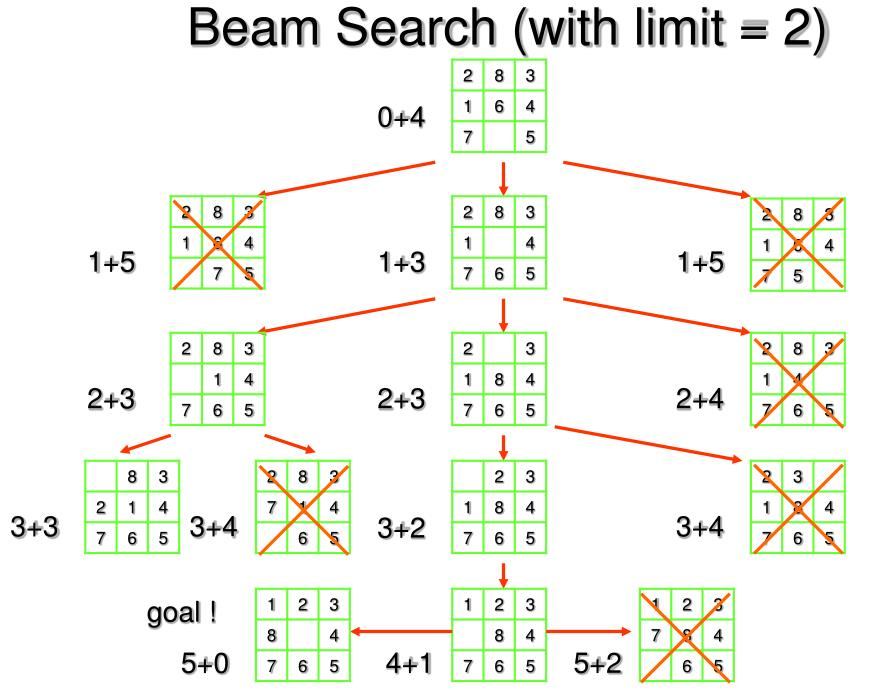
\includegraphics[width=0.8\textwidth]{source/local-beam-example.png}
    \label{fig:beam-search-example}
\end{figure}
